% \documentclass[12pt,openright,oneside,a4paper,brazil]{abntex2}
% \usepackage[utf8]{inputenc}
% \counterwithout{section}{section}
% \counterwithout{figure}{chapter}
% \counterwithout{table}{chapter}
% \setlength{\parindent}{1.3cm}
% \usepackage{indentfirst}
% \setlength{\parskip}{0.2cm}
% \usepackage[bottom=2cm,top=3cm,left=3cm,right=2cm]{geometry}
% \usepackage{graphicx}
% \graphicspath{{figuras/}}
% \usepackage{placeins}
% 
% %opening
% \title{}
% \author{}
% 
% \begin{document}

%capa

% \textual
\begin{center}
 {\large Declaração de escopo}\\[0.2cm]
 {Planta de abastecimento de água potável a partir da umidade do ar}\\
 \end{center}
 
 \section*{Histórico de Alterações}
\begin{table}[h]
\centering
\begin{tabular}{|c|c|p{6cm}|p{5cm}|}

\hline
Data & Versão & Descrição & Responsável\\
\hline                               
21/04/2015 & 0.0 & Criação do documento. & César A. Marques Jr., Jonnatas L.L. Costa\\
\hline
22/04/2015 & 1.0 & Alteração dos itens: III, VII e IX & Jonnatas L. L. Costa\\
\hline
22/04/2015 & 1.1 & Alteração dos requisitos & Jonnatas L. L. Costa\\
\hline
\end{tabular}
\end{table}

\section*{Nome do projeto}
  Planta de abastecimento de água potável a partir da umidade do ar
  
  \section*{Descrição do projeto}
O projeto visa desenvolver uma planta de abastecimento de água potável, por meio de um sistema de captação a partir da umidade do ar na cidade de Aracari-RN (município da Microrregião do Seridó Oriental, na região do Seridó), no bairro Vereador Tarcísio Bezerra Galvão. O bairro possui uma população de aproximadamente 900 habitantes e sofre constantemente com a falta de água. 
O projeto gira em torno de uma solução tecnológica  capaz de retirar a água do ar e por processos químicos e físicos e tornar essa água potável e própria para o consumo humano de forma renovável e menos danosa possível. Para isso aplicamos conhecimentos das demais áreas da engenharia atuando no desenvolvimento e conceituação do projeto. Nossa estimativa é de que possamos produzir aproximadamente 3 mil litros de água por dia. Essa quantidade e suficiente para atender toda a população do município. 
O projeto conta com grupos que trabalham em áreas diferentes mas interligadas e com um único propósito. Cada etapa e gerida e coordenada por representantes de forma a garantir um resultado rápido e com qualidade.


\section*{Objetivos do projeto}
  
  Este trabalho tem por objetivo propor um projeto de solução que consiga suprir a demanda da população. Os esforços que serão
realizados ao longo do período de desenvolvimento, no transcorrer de todas as etapas do processo buscam a qualidade e real
eficácia do produto, ou seja, oferecer a demanda de água do bairro Vereador Tarcísio Bezerra Galvão situado em Aracarí-RN, 
água potável de qualidade.

 São objetivos específicos do projeto:
 \begin{itemize}
  \item Elaborar o projeto mecânico estrutural do sistema de captação de água;
  \item Elaborar o projeto estrutural do sistema de transporte da água para a central de armazenamento;
  \item Elaborar o projeto do sistema de monitoramento e controle da qualidade da água captada;
  \item Elaborar o projeto da matriz energética que dará o suporte para os sistemas de captação de água e monitoramento e controle;
 \end{itemize}
  
\section*{Justificativa do projeto}
 \begin{enumerate}[label=\Alph*]
\item Por que deve-se pensar em projetos como esse?\\
Atualmente, cerca de 40 \% da população mundial sofre com consequências da falta de água, além da sede faltam recursos hídricos, o que gera graves implicações na economia e política. De acordo com o geólogo Sjiklomanov, do Instituto Hidrológico Estadual de São Petesburgo, Rússia, em 2000 foi previsto que: “Os países em desenvolvimento vão aumentar seu uso de água em até 200\% em 25 anos”. Em 2014 no Brasil, foi evidenciado consequências desse aumento no consumo de água juntamente com fatores climático, resultando na falta de água em cidades de Pernambuco, Minas Gerais e São Paulo.
Essa situação de falta de água não é nova, a ONU em 2003 já previa os futuros transtornos que seriam causados pela crise de água. O World Water Development Report, se destaca sobre o tema porque é um documento da ONU que também traz estudos mostrando como esse problema já afeta e mata milhares de pessoas. Este estudo prevê que 2,7 bilhões de seres humanos – 45\% da população mundial – vão ficar sem água no ano 2025.
Diante dessa situação e de previsões sobre a falta de água tão breves, devem-se tomar medidas para minimizar a situação e planejar soluções para a produção de água potável buscando outras fontes, como o ar, por exemplo. Por isso, esse projeto visa através da umidade do ar, retirar água potável e planeja um estudo de abastecimento na cidade de Acari, RN.

\item Por que  Aracarí foi a cidade escolhida?\\
Na situação de crise hídrica vivida pelo país atualmente, observa-se grandes centros urbanos sofrendo com a falta de água para consumo humano (o que antes era praticamente exclusivo para a região do semiárido nordestino). Além disso, observa-se que a seca na região nordeste vem se agravando muito nos últimos anos, especificamente na região do Seridó, que fica no semiárido do RN.
Dessa forma, soluções alternativas para o abastecimento de água potável a fim de atender o consumo humano fazem-se necessárias. Sendo assim, a região para a qual o sistema será projetado será o município de Acari – RN, pois é uma região onde há muita demanda (11303 habitantes) e tem sofrido muito com a escassez de água. A escolha dessa região baseia-se principalmente na questão social, uma vez que o projeto visa atender o consumo humano de pessoas que não tem acesso à água potável.
Além de ser uma região que apresenta necessidade de um planejamento para a amenização ou suprimento da escassez de água, é também, uma região muito quente com temperatura média anual de 33Cº, pois está localizada no polígono das Secas (local de maior concentração de seca no país). Consequentemente, o volume de água do Açude de Gargalheiras, açude este que abastece a cidade, decai consideravelmente em épocas de seca, fazendo com que haja escassez de água na cidade. A possibilidade de retirar água potável do subterrâneo, é inviável pois a água é muito salobra. Apesar de clima quente e semi-árido a umidade do ar nessa região  possui uma média anual de 60\%, o que possibilita a implantação de tecnologias que retiram a umidade do ar  e transforma em água potável. Portanto, devido a esses fatores apresentados, a cidade foi escolhida para se realizar o planejamento.

\item Por que se escolheu o bairro Vereador Tarcísio Bezerra Galvão?\\
De acordo com o censo 2010 o bairro Vereador Tarcísio Bezerra Galvão tem cerca de 900 habitantes onde a maioria, cerca de 60\%, possui entre 15 e 64 anos. Sua localização foi uma das principais motivações para a escolha do bairro, pois é um bairro muito próximo do Açude de Gargalheiras, e uma das áreas a ser planejada nesse projeto é em relação à distribuição da água, ou seja, o açude pode facilitar essa distribuição. Outro motivo seria para limitar um pouco mais o projeto a uma população menor, para assim agilizar e facilitar o estudo para planejamento.
\end{enumerate}
  
\section*{Produtos do projeto}

  O presente trabalho fornecerá os seguintes produtos:
  
  \begin{itemize}
    \item Projeto estrutural mecânico das unidades de captação de água da umidade do ar.
    \item Projeto estrutural do sistema de transporte da água para a central de armazenamento.
    \item Projeto do sistema de monitoramento e controle da qualidade da água captada.
    \item Projeto da matriz energética que dará o suporte para os sistemas de captação de água e monitoramento e controle.
  \end{itemize}

\section*{Critérios de aceitação do produto do projeto}

  Os produtos de projeto devem atender as especificações inerentes aos requisitos funcionais
  e não-funcionais de cada produto específico.
  
\section*{Exclusões específicas e limites do projeto}

  Ficam excluídos das competências do projeto:
  
  \begin{itemize}
   \item Atividades como as de tratamento de recursos hídricos já existentes na região e que não possuem
      as especificações mínimas para consumo humano, como é o caso da água salobra.
   
   \item Todo o processo de manutenção dos componentes do sistema, visando uma durabilidade de longo prazo, não fará parte 
      do escopo deste projeto. Também não fará parte do escopo a distribuição de água para localidades vizinhas.
      
   \item O uso de tecnologias auxiliares para a obtenção da água, como é o caso osmose reversa, não serão abordadas
      pois fogem da premissa inicial.
   
   \item O tratamento da energia residual gerada.
   
   \item O tratamento da água residual que for armazenada nos tanques.
   
  \end{itemize}

\pagebreak
\section*{Estrutura Analítica do Projeto}

  \begin{figure}[h]
  \begin{center}
    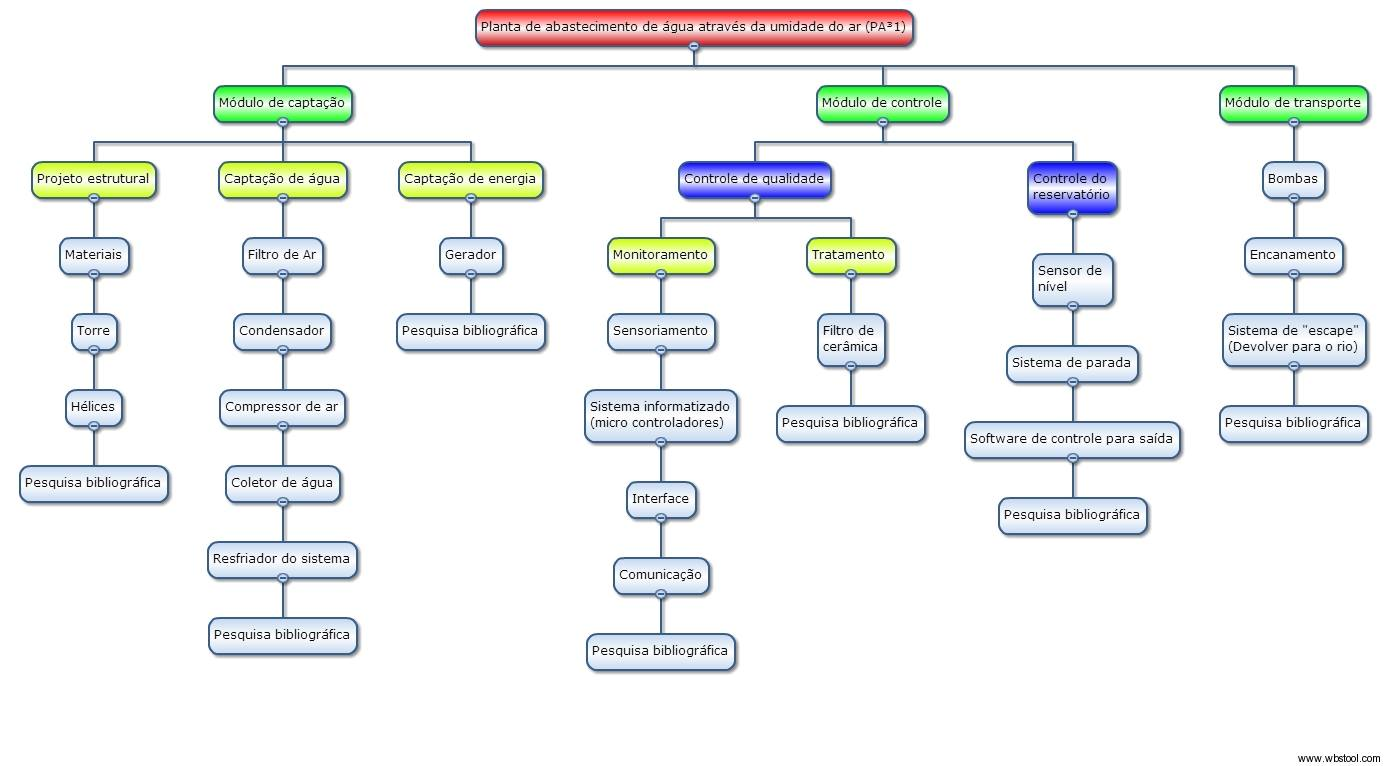
\includegraphics[scale=0.3]{editaveis/figuras/EAP}
    \label{EAP}
  \end{center}
  \end{figure}
  \FloatBarrier
  
\section*{Características e requisitos do produto do projeto}

  Os produtos do projeto são partes que compõem um sistema que tem por características principais ser um sistema auto sustentável
  e que não seja muito agressivo ao meio ambiente, utilizando uma matriz energética alternativa.
  A estimativa é que o produto gere cerca de 3 mil litros de água potável por dia.
  
  O sistema conta com uma central de monitoramento para garantir a qualidade da água produzida. Possui uma série de sensores
  com funções variadas, que vão de ler a umidade do ar até a medição de dados sobre a água.
  
  Uma importante característica do sistema é que ele pode se adequar às mudanças climáticas, de forma que ele pare de
  funcionar quando a umidade do ar chegar a um nível mínimo, para que não afete a saúde da população.
  
  O projeto possui quatro frentes de requisitos:
  
    \begin{itemize}
      \item Requisitos do projeto estrutural mecânico do sistema de captação da água e do transporte para a central de armazenamento;\\
	
	\textbf{Requisitos funcionais}
	  \begin{itemize}
	   \item Retirar água da umidade do ar;
	   \item Bombear água para o reservatório;
	  \end{itemize}
	  
	  \textbf{Requisitos não-funcionais}
	  \begin{itemize}
	   \item O sistema deve atender a uma demanda de água diária;
	   \item O sistema deve bombear toda água por dia produzida pro reservatório; 
       \item O sistema deve ser composto por materiais resistentes à água;
       \item O sistema deve possuir um reservatório de capacidade de até 3 dias de água;
       \item O sistema deve operar com incidências de ventos de 7 a 50 m/s, umidade a partir de 40\% e 	temperatura à partir de $26\,^{\circ}\mathrm{C}$\cite{eole}
       \item O sistema deve aproveitar o relevo da região para o transporte da água;

	  \end{itemize}
	
      \item Requisitos do projeto dos circuitos eletrônicos que irão compor o sistema de monitoramento e controle da qualidade da água.\\
	
	\textbf{Requisitos funcionais}
	\begin{itemize}
	  \item Atuar como um sistema de controle dos elementos do sistema de modo a produzir a saída desejada (manter a água própria para o consumo humano);
	  \item Obter informações climáticas da região;
	  \item Obter dados do estado reservatório;
	  \item Ler parâmetros que definem a qualidade da água;
	  \item Efetuar conversão analógica/digital dos sinais filtrados;
	  \item Processar o sinal convertido de modo que os dados possam ser transmitidos ao usuário;
	  \item Exibir dados obtidos ao usuário;
	\end{itemize}
	
	\textbf{Requisitos não-funcionais}
	\begin{itemize}
	  \item Utilizar sensores para obtenção dos dados;
	  \item Exibir dados dos sensores ao usuário em tempo real;
	  \item Utilizar filtros analógicos para retirar eventuais ruídos que a saída do sensor possa gerar;
	\end{itemize}
	
      \item Requisitos do projeto do sistema de Gestão da Informação do monitoramento da qualidade da água;\\
	 
	 \textbf{Requisitos funcionais}
	  \begin{itemize}
	   \item Apenas o moderador poderá, modificar os dados.
	   \item O sistema registrará os dados de qualidade da agua.
	   \item O sistema deve emitir um alerta caso um parâmetro de qualidade não esteja aceitável.
	   \item O sistema deve permitir consultas dos dados armazenados de datas anteriores.
	   \item O sistema deve possuir uma interface pare exibir os dados.
	   \item O sistema deve possuir uma página de \textit{login} antes de entrar no sistema.
	   \item O sistema deve possuir um mecanismo de impressão dos dados.
	   \item O sistema possuirá um mecanismo para exportar os dados.
	  \end{itemize}
	  
	  \textbf{Requisitos não-funcionais}
	  \begin{itemize}
	   \item O sistema deve ser fácil de usar, evitando excesso de digitação, de modo a dar agilidade ao processo.
	   \item O sistema deve possuir uma interface simples.
	   \item O sistema deve funcionar no sistema operacional Windows.
	   \item O sitema deve monitorar as amostras de água a cada 30 mimutos.
	  \end{itemize}
      
      \item Requisitos do projeto da matriz energética que dará o suporte para o sistema de captação de água e o sistema de monitoramento da qualidade da água;\\
      
	\textbf{Requisitos funcionais}
	\begin{itemize}
	  \item Produzir energia elétrica através da energia eólica;
	  \item Converter energia cinética em energia elétrica;
	  \item Armazenar a energia elétrica gerada;
	  \item Fornecer energia para os componentes eletrônicos, de controle e monitoramento do produto final;
	  \item Fornecer energia para o bombeamento mecânico de água.
	\end{itemize}
	
	\textbf{Requisitos não-funcionais}
	\begin{itemize}
	  \item Utilizar uma fonte renovável de energia;
	  \item Ser autossuficiente no quesito energia gerada-consumida;
	  \item Possuir eficiência energética aceitável;
	  \item Ser estável energeticamente;
	\end{itemize}
	
    \end{itemize}
  
\section*{Assinaturas}

  \begin{center}
  Data: \rule{0.5cm}{0.1mm}/\rule{0.5cm}{0.1mm}/\rule{1cm}{0.1mm}     \\
  \rule{13cm}{0.1mm}\\
  ADRIANNY VIANA DE ARAÚJO AMORIM – GERENTE DE PROJETO\\


\end{center}
% \end{document}